\chapter{Git——程序和文档的版本管理}
\section{学习参考资料}
\begin{itemize}
\item Git 官网:\url{http://git-scm.com}

\item Github 官网:\url{https://github.com}

\item 廖雪峰个人网站:\url{http://www.liaoxuefeng.com} 对Git的作用,历史,诞生都讲的比较清楚,入门很有用。

\item 视频解说参考:Bilibili 搜索git,如\href{https://www.bilibili.com/video/BV1pW411A7a5?from=search&seid=3815767452396308043}{尚硅谷官方}、庄七。
\end{itemize}


\section{推荐的学习步骤与目标}
\begin{itemize}
\item 先看尚硅谷的git\&github视频教程1-42集,目标:
	\begin{itemize}
	\item 做好笔记;
	\item 完成git的安装;
	\item 基本操作跟随视频演练一边;
	\item 注册github账户
 	\end{itemize}
\item Fork本文档 \url{https://github.com/xuanleng/SiSR},建立本地库
\item 并推送一条修改。修改内容为:编辑本文档“前言”章节中“第一次推送打卡”小节,记录下自己的第一次推送和感言。
\item 由于本章节是文档协作之本,希望大家踊跃补充本章节忽视的内容。目标是,在看完推荐视频后,所有不熟悉的git相关操作都能在本章节中找到,不需要再花时间找第三方资料。
\end{itemize}


\section{基本思想和历史}
以我们的量子耗散动力学、光谱计算为例
\begin{enumerate}
\item 找个合适的模型作为标准模型;
\item 只要新增内容,就新复制一个,说明改进;
\item 所有新功能先在标准模型上实现,再应用;
\item 结合git版本控制。
\end{enumerate}


Git基本概念
\begin{itemize}
\item 本地电脑
\begin{itemize}
\item 工作区:写代码
\item 暂存区:临时存储
\item 本地库:历史版本
\end{itemize}

\item 远程服务器:远程仓库(与别人共享)
\end{itemize}






\section{软件安装}
\subsection{Linux版本安装}
\subsection{Windows版本安装}


\section{配置与操作}
\subsection{初始化}
\begin{itemize}
\item[(1)] 本地库初始化(建立本地库)
\begin{itemize}
\item git init\\
进入项目目录,在命令行输入 git init,会产生一个.git的子目录,存放的是本地库相关的目录和文件,不要删除和胡乱修改。
\end{itemize}

\item[(2)] 设置签名
\begin{itemize}
\item git config user.name XX
\item git config user.email XX
\end{itemize}

\item [(3)] 配置
\begin{itemize}
\item \verb|git config --global core.editor  "vim"| : 使用Vim作为编辑器
\end{itemize}

\end{itemize}



\subsection{提交}
\begin{enumerate}
\item git status: 查看状态
\item \verb|git add <file>|: 添加追踪文件到缓存区 
\item  \verb|git rm --cached <file>| :移除缓存区追踪文件
\item \verb|git commit <file>|:提交文件到库
\item \verb|git commit -a |:直接将所有修改文件提交到库(也可以分成两步,先git add更新缓存区,再git commit提交到库)
\item \verb|git commit -m ``xxx'' <file>|:跳过消息编辑器步骤,直接提交“xxx”更新记录
\item \verb|git commit -a -m ``xxx''|:综合前两个命令
\end{enumerate}



\subsection{版本穿梭}
\begin{enumerate}
\item \verb|git reflog|:精炼形式历史记录查询。完整形式:\verb|git log| 

\item \verb|git reset --hard <index>|:历史版本选择\\
注意,还有其他两个参数\verb|--soft|、\verb|--mixed|。基于这个功能,可以实现删除文件并找回,但前提是文件存在时的状态必须提交到了本地库。
\end{enumerate}



\subsection{比较文件差异}
\begin{enumerate}
\item git diff <file> :将工作区中的文件和暂存区进行比较
\item git diff <本地库中某个历史版本> <file>:将工作区中的文件和本地库中历史文件进行比较
\item 不带文件名则比较多个文件
\end{enumerate}



\subsection{分支管理}
\begin{enumerate}
\item \verb|git branch -v |:查看分支
\item \verb|git branch <name>| :创建分支
\item \verb|git checkout <name>|:切换分支
\item 合并分支
\begin{itemize}
\item 切换到要合并到的分支
\item \verb|git merge <branch name>|:
\end{itemize}
\item 解决合并冲突
\begin{itemize}
\item  编辑文件,删除特殊符号
\item 把文件修改到满意的程度,保存退出
\item \verb|git commit -m | ``日志信息''。注意此时不能带文件名。
\end{itemize}
\end{enumerate}



\section{远程仓库Github/Gitee/Gitlab}
网上的git远程仓库很多,但是操作流程基本一样。这里以Github为主,Gitee可以参考:\url{https://www.bilibili.com/video/BV1mb411n7Nw?p=4}


\subsection{协作基本流程}
\begin{figure}[h!]
\centering
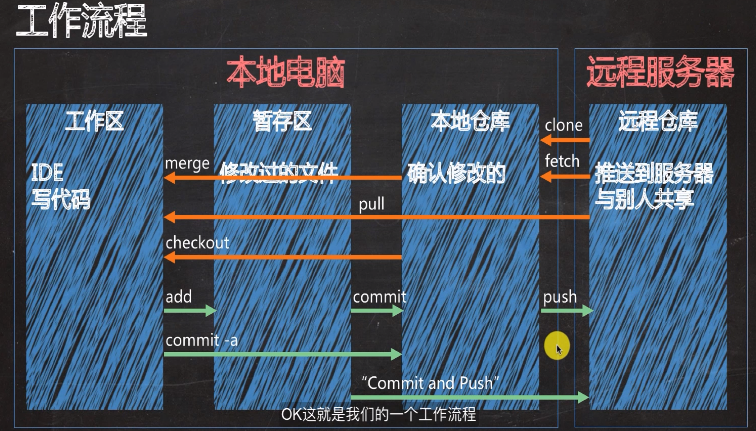
\includegraphics[width=0.9\textwidth]{pictures/git.png}
\caption{Git 工作流程\footnote{\url{https://www.bilibili.com/video/BV1mb411n7Nw?p=3}}}
%\label{fig:by:table}
\end{figure}

\begin{enumerate}
\item  主管人创建主远程仓库。
\item 协作人克隆主远程仓库,并拉取到本地。
\item 协作人在本地修改,上传到协作人的克隆远程仓库。
\item 协作人立即(或积累一定程度后),回到主远程仓库网页上,通过 Github 页面提交 pull requests。
\begin{itemize}
\item 首先,找到绿色的 New pull requests 按钮并点击,然后点击图中的 compare across forks;
\item 选择要提交的内容,通过比较文件差异,确认无误之后,点击绿色的eate pull request 即可。
\end{itemize}
\item 主管人在接到推送通知后,首先保证自己本地库与主远程仓库一致,否在合并时仍需回到这一步。
\item 主管人拉取协作人的远程仓库到本地,形成一个分支。
\item 主管人合并协作人的分支到主分支上。
\item 主管人再将合并后的最新版本推送到主远程仓库,至此完成一次协作。
\end{enumerate}
注意:无论是创始人还是协作人的远程仓库和本地库,都是相互独立的。


\subsection{创建远程仓库}
注册账户,在网页上创建。需要注意的是,在网页上创建通常会辅助产生一些文件,与本地库产生一些冲突。如两个分支是不同的版本,具有不同的提交历史。这时需要不相关历史强制合并:
\verb|git pull origin master --allow-unrelated-histories |



\subsection{推送到远程仓库}
\url{https://www.bilibili.com/video/BV1pW411A7a5?p=35}
\begin{itemize}
\item \verb|git remote -v|:查看远程库
\item \verb|git remote add <name> <https://address> |:添加远程库地址别名(name)
\item \verb|git push <name> <branch>|:推送分支
\end{itemize}

\subsubsection{ssh免密推送设置}




\subsection{拉取和获取远程仓库}
\begin{itemize}
\item git pull:从远程仓库拉取最新版本到本地,并自动合并。
\item git fetch:从远程仓库获取最新版本到本地,但不会自动合并。
\end{itemize}


\subsection{主分支合并}
例如:
\begin{itemize}
\item[Step 1:] From your project repository, check out a new branch and test the changes.
\begin{enumerate}
\item git checkout -b Limingtan11-master master

\item git pull https://github.com/Limingtan11/SiSR.git master
\end{enumerate}

\item [Step 2:] Merge the changes and update on GitHub.
\begin{enumerate}
\item  git checkout master

\item git merge --no-ff Limingtan11-master

\item git push origin master
\end{enumerate}
\end{itemize}








\subsection{邀请合作者}
\begin{enumerate}
\item 进入自己的远程仓库主页,点击“Settings”;
\item 点击左侧“Options”栏目下的“Manage access”;
\item 就可以用“用户名”、“邮箱”等形式邀请了。
\end{enumerate}




\chapter{\LaTeX{}——编译型文档排版系统}
\section{学习参考资料}
\begin{itemize}
\item 安装: 啸行,一份简短的关于\LaTeX{}安装的介绍,\url{https://github.com/OsbertWang/install-latex}
\item 介绍:\url{http://mirror.utexas.edu/ctan/info/lshort/chinese/lshort-zh-cn.pdf}
\item 指南:\url{https://www.tug.org/texlive/doc/texlive-zh-cn/texlive-zh-cn.pdf}
\end{itemize}


\section{基本思想和历史}
我觉得它与Word的最大不同,应该是输入的方式了。它是靠直接“说”来代替Word中的那些不断缓慢的操作。比如:Word中改变字的颜色,是靠操作来完成的,选则相应的文字,然后去点击一些操作图标。而它是在要改变颜色的那段直接写上“换成某某颜色”的命令。这样书写公式就很简单,它可以像我们读公式一样,直接输上去就行了。比如$\sqrt{2}$,它可以直接输类似“根号2”的命令,即:\verb|$\sqrt{2}$|。也就是说一切操作只靠键盘就可以完成,甚至鼠标都不用点。这样是极大提高工作效率。对于那些老手来说,一路敲过去,转换出来就是漂亮的排版了。这样输公式爽多了。但要记住一堆命令。初学起来就不习惯了。

但是我觉得这还是个历史产物。以后随着技术不断先进,手写功能越来越强大,将是与手写识别相结合的情况。直接手写输入公式,就可以转换成自己想要的效果。对于一些微调又可以用命令来做。

\rightline{——冷轩\qquad}



\section{主体发行版——\TeX{} Live }
\subsection{Win10下安装}
注意要点:
\begin{itemize}
\item 全部安装占用空间比较大,。。。
\item 手动添加编译器路径到路径环境变量:
This PC->Advanced system settings->Advanced->Environment Variables...(右下角)->System variables->Path,点开。添加C:/texlive/2020/bin/win32。大家安装的路径可能不一样,但是选择\LaTeX{}相关编译器的路径就行。要点是,一定是编译器所在路径,上一级都不行。
\end{itemize}



\subsection{Ubuntu下安装}
(1)下载镜像
直接下载DVD光盘镜像的。不建议网络安装。官网主页:\url{http://www.tug.org/texlive/}


(2)安装
\paragraph{(a)文字界面安装}
%安装过程我没用图形界面,因为图形界面还要先安装一个包,觉得麻烦。
文字界面也简单,在终端中运行 Perl 脚本install-tl。 这就是在终端中运行一个文件。 运行一个文件, 当然需要告诉电脑文件在哪里了,于是在终端输入该脚本的全路径就行了,如:\\
\verb*|perl /home/phileas/texlive/install-tl|\\
或先转到相应的目录下,再执行,如:\\
\verb*|cd /home/phileas/texlive|\\
\verb*|perl install-tl|

运行后,会出现各种选项和提示。可以看到,texlive是装在文件系统中的,你可以更改安装的路径,或开启终端中的超级用户的权限,再来运行这个脚本。开启超级用户权限的方法是:在终端中输入命令:sudo -i。这样就可以安装了。

\paragraph{(b)图形界面安装}
建议使用图形安装界面,因为宏包用图形界面管理很方便,过程如下:
\begin{enumerate}
\item \verb*|sudo -i| 开启超级用户权限,这是因为默认安装到文件系统中,而改动文件系统是需要超级用户权限的,也可以不开启,到时选个可以安装的路径就行了。
\item  \verb*|apt-get install perl-tk| 安装 perl-tk 包才能用图形安装界面
\item 挂载镜像\\
先将光盘镜像挂载到一个文件夹中,如:/home/phileas/texlive,意思是:根目录/下的home文件夹phileas中的texlive文件夹。先找出光盘镜像的全路径,很简单,选中你的光盘镜像右键属性中有写,这个路径或许当你拷贝进这个文件时你就已经知道了,我放的位置是,\\
/home/phileas/desktop/texlive2011-20110705.iso,
最后一项是该文件名。挂载方法是在终端中,敲命令:\\
sudo mount /home/phileas/Desktop/texlive2011-20110705.iso/~~ /home/phileas/texlive ,
注意两个路径之间有空格。这样就挂载好了。(注意路径区分大小写)
\item cd挂载的镜像文件夹下,终端输入perl install-tl  - -gui
\item 有些选项,自己看着办。注意勾选建立符号链接(symbol link),很简单,勾选上就有了,不建立这个,之后在终端开启图形管理宏包界面的命令tlmgr - - gui就会报错说没有这个命令,其实还是要再加链接。所以这里记得勾选。(安装时没勾选也没关系,这部分内容在texlive相应版本的说明文档中说的很清楚。)
\item 点击安装

\item 如果安装时忘了勾选符号链接,则需添加环境变量。在\verb|~/.bashrc|文件中添加\\
\verb|export PATH=$PATH:/usr/local/texlive/2018/bin/x86_64-linux|\\
\verb|export MANPATH=$MANPATH:/usr/local/texlive/2018/texmf-dist/doc/man|\\
\verb|export INFOPATH=$INFOPATH:/usr/local/texlive/2018/texmf-dist/doc/info|\\
然后在终端中使环境变量生效:\\
\verb|source ~/.bashrc|

\item 调出图形管理宏包界面,在终端输入tlmgr - -gui,这时要改宏包更新源,在option选项改成网络为默认更新源。不然还是更新不了。
\end{enumerate}




\section{Texworks}
注意:有时候Texworks没有自动找到\LaTeX{}相关编译器的路径。这时需要手动添加
Edit->Perference->Tyepsetting,添加
C:/texlive/2020/bin/win32(win10系统)。要点是,一定要是编译器所在目录,上一级都不行。


\subsection{安装}
官网:\url{https://www.tug.org/texworks/}\\
\verb|sudo add-apt-repository ppa:texworks/stable|\\
\verb|sudo apt-get update|\\
\verb|sudo apt-get install texworks|


\subsection{简述}
[转] \url{http://blog.sina.com.cn/s/blog_630306a50101fjwy.html}

Texworks 是目前我用的最多的\LaTeX 编辑软件,不是跟 ddswhu 交流,我还一直不知道,里面还蕴含着很多方便快捷的缩写。这里就是主要谈谈这些快捷缩写。这些缩写都在一个叫completion 的文件中,到 Texworks 安装目录下找找。

首先,对 TeXworks 的自动补全功能解释一下:

1、在 TeXworks 的编辑窗里面键入 xa,按下tab,出现了 \verb|\alpha|,这就是最简单的补全,对简单命令的补全。

2、在 TeXworks 键入usep,按下tab建,得到了 \verb|\usepackage{}|,这就是最普通的补全,给出命令后的必须参数括号,并且光标停留在括号内。

3、在TeXworks键入usepo,按下tab,得到了 \verb|\usepackage[]{•}|,这是对含有可选参数的命令的补全,光标停在可选参数的中括号内,当我们把可选参数补完之后,按下ctrl+tab组合键,光标进入后面的必需参数括号内(后面的位置称为placeholder)。其中ctrl+tab是移向往下最接近的一个placeholder,shift+tab是移向往上最近的一个placeholder。
 
在刚才的例子中,我们只按了一次tab,假如我们键入的引导词是若干个命令的引导词的前部分,则继续按下tab键会在这几个命令中切换,得到你想要的命令。
 
好了,为了使用自动补全,我们需要记住引导词。在TeXworks中,已经定义了很多的引导词,而且也允许用户自己定义新的引导词。
 
下面对常用的引导词归类。
 
\subsection{环境类}
对于环境的补全,引导词第一个字母均为b,后面字母个数不定,但是,对绝大多数的环境,只需要使用环境名的前三个字母就行,即为"b+xyz+[tab]"。
 
比如 itemize 环境,根据规则,我们需要键入 "bite",然后按下tab键,即得到了
\begin{verbatim}
\begin{itemize}
\item
 
\end{itemize}•	
\end{verbatim}

符合此规则的环境有document,abstract,align,tabular,appendix,bmatrix,pmatrix,cases,
description,center,equation,enumerate,eqnarray,figure,flalign,
gather,item,letter,list,minipage,multiline,picture,split,subequations,
theorem,titlepage,trivlist,varwidth,verbatim,等。
 
注意事项:如果环境名开头带有the,则xyz为除去the之后的环境名的前三个字母。比如bind=theindex环境、bbib=thebibliography环境。
 
另外需要注意的是:星号环境在原来引导词后加s,即为"b+xyz+s+[tab]",如果环境有可选项,需要使用可选项,则需要在末尾加上o(option的意思),即为"b+xyz+o+[tab]"。
 
几个特殊的环境:

align    :b+ali(s)
alignat   :b+ali+at(s)
aligned  :b+ali+ed
alignedat :b+ali+edat(o)
 
verbatim  :bver
verse    :bvers
tabular   :b+tab
tabularx  :b+tabx
tabbing  :b+tabb
table    :b+tabl、b+tbl (s,o,so)
 
居左、居右环境、居中
flushleft+flushright :b+fl+l/r
\verb|\centering|         : cen
 
 
 
 \subsection{字体}
(1)普通字体命令

(1.1)\verb|\textbf, \texttt, \textsf, \textsc, \textsl, \textit, \textup|

   方法一、由字体属性的两个关键字构成,比如 sc+[tab键],textit有问题,em表示\verb|\emph{}|
   
   方法二、\verb|\text(b/t/s/i/w...)+[tab键]|
   
   注意:\verb|\textwidth| 也是 \verb|\textw|

(1.2)属性的第二种表示方式、"属性关键字+d"

    bfd: \verb|\bfseries|
    ttd: \verb|\ttfamily|
    sfd: \verb|\sffamily|
    scd: \verb|\scshape|
    sld:  \verb|\slshape|
    itd:  \verb|\itshape|
    upd: \verb|\upshape|
    emd: \verb|\em|
 
(2)数学字体命令:
    
  \verb|\mathbf, \mathrm, \mathcal, \mathsf, \mathtt, \mattit|
  
    引导词为"m+字体属性关键字"。比如:mbf\verb|\mcal|
 

 
 \subsection{希腊字母类}
方法:”x+[c(大写符号)]+符号首字母”

适用的字母有:
\begin{verbatim}
\alpha, \beta , \chi, \delta, \gamma, \Gamma, \iota, \mu, \lambada,
\Lambda, \mu, \nu, \omega, \Omega, \pi, \sigma, \zeta, \rho, \tau,
\upsilon, \xi, \Xi
\end{verbatim}

注意以下相同首字母的写法(特殊):

\verb|\epsilon|: x+e
\verb|\varepsilon|: x+v+e
\verb|\eta|: x+et
\verb|\phi| :x+p
\verb|\varphi| :x+v+p
\verb|\phi| :x+ph
\verb|\Phi| :x+c+ph
\verb|\varphi| :x+v+ph
\verb|\psi| :x+ps
\verb|\Psi| :x+c+ps
\verb|\tau| :x+t
\verb|\theta| :x+th
 
 
 
 \subsection{章节命令}
cha     =\verb|\chapter{}|

sec(o)   =\verb|\section{}|

ssec(o)  =\verb|\subsection{}|

sssec(o) =\verb|\subsubsection{}|

 
\subsection{参考文献}
bbib      =\verb|\begin{thebibliography}|
bibitem   =\verb|\bibitem|
bibitemo  =\verb|\bibitem[]|
bibstyle   =\verb|\bibliographystyle{}|
biblio     =\verb|\bibliography{}|
 
  
 \subsection{杂项与普通命令}
1、括号

dd : \verb|\( \)|

\verb|d+希腊字母表达式=\(希腊字母\)|

例如:dxa = \verb|\(\alpha\)|
 
2、普通命令

usep   =\verb|\usepackage{}|

foot    =\verb|footnote foot|

frac    =\verb|\frac|

fbox   =\verb|\fbox|

fboxo  =\verb|\framebox|

href   =\verb|\href|

incg   =\verb|\includegraphics{}|

incgo  =\verb|\includegraphics[]{•}|

ncol(newcolumn) = \verb|&|

newc  =\verb|\newcommand{}{•}|

newe  =\verb|\newenvironment{}{•}{•}|

newpg =\verb|\newpage|

pgref  =\verb|\pageref{}|

pgs   =\verb|\pagestyle{}|

sqrt   =\verb|\sqrt{}|

toc   =\verb|\tableofcontents|

listf   =\verb|\listoffigures|

list   =\verb|\listoftables|
multic =\verb|\multicolumn{}{•}{•}|



%\section{Sublime Text}




\chapter{科研入门技能及心得}
\section{科研导师的选择}
\begin{enumerate}
\item 必须步骤:人品和性格匹配调查,可靠来源为现任组里成员,最好为新老成员。
\end{enumerate}


\section{一些该注册的}
\subsection{Gmail}
 至少申请两个,一个注册用,一个通讯用(真名)。

\begin{itemize}
\item Gmail查看所有未读邮件\footnote{\url{https://jingyan.baidu.com/article/cbcede0761144902f40b4d18.html}}:
\begin{enumerate}
\item 打开登陆Gmail网页,在主界面点击上面的搜索框的下拉选项;
\item 弹出下拉窗口,在第一行点击搜索所有邮件,然后在下拉选项中选择未读邮件,只搜索未读邮件;
\item 然后日期范围选最大的,选一年,然后点击搜索,意思就是搜索一年内所有未读邮件。
\end{enumerate}
或者
\begin{enumerate}
\item 打开Gmail网页,在搜索框中输入代码“is:unread ”
\end{enumerate}
\end{itemize}



\subsection{Google Scholar}


\subsection{Research gate}


\subsection{OCRC}




\section{文献管理、检索与推送}
文献是科研之魂,高效管理文献是科研的第一步——冷轩 \quad 语 (这里的文献特指期刊论文)
\subsection{文献管理的基本思想}
\begin{itemize}
\item 平等的看待每一篇文献。不需要专门的、特别的去存储某些文献。文献的时效性太短了,发现多年前的Nature、Science 正刊等对现在没有任何参考意义。

\item 文献多元分类。每篇文献有不同的标签。

\item 文献不同平台、设备的同步。常见的应用场景是,工作电脑下载了文献,然后用带手写笔的设备去细看、标记。
\end{itemize}
仅仅靠本地创建文件夹的方式去管理,是非常不方便的。需要采用专业的文献管理软件,非常推荐Zotero。





\subsection{免费文献管理工具——Zotero}
参考资料:
\begin{itemize}
\item 青柠学术微信公众号的专辑“Zotero|打造最佳文献生态”(由于网络链接比较繁杂,请自行搜索)
\item \url{https://zhuanlan.zhihu.com/p/28325366}
\end{itemize}


Zotero (\url{https://www.zotero.org/}) 是一款免费、跨平台并且强大的文献管理工具,如图(\ref{fig566})所示。
\begin{figure}[h!]
\centering
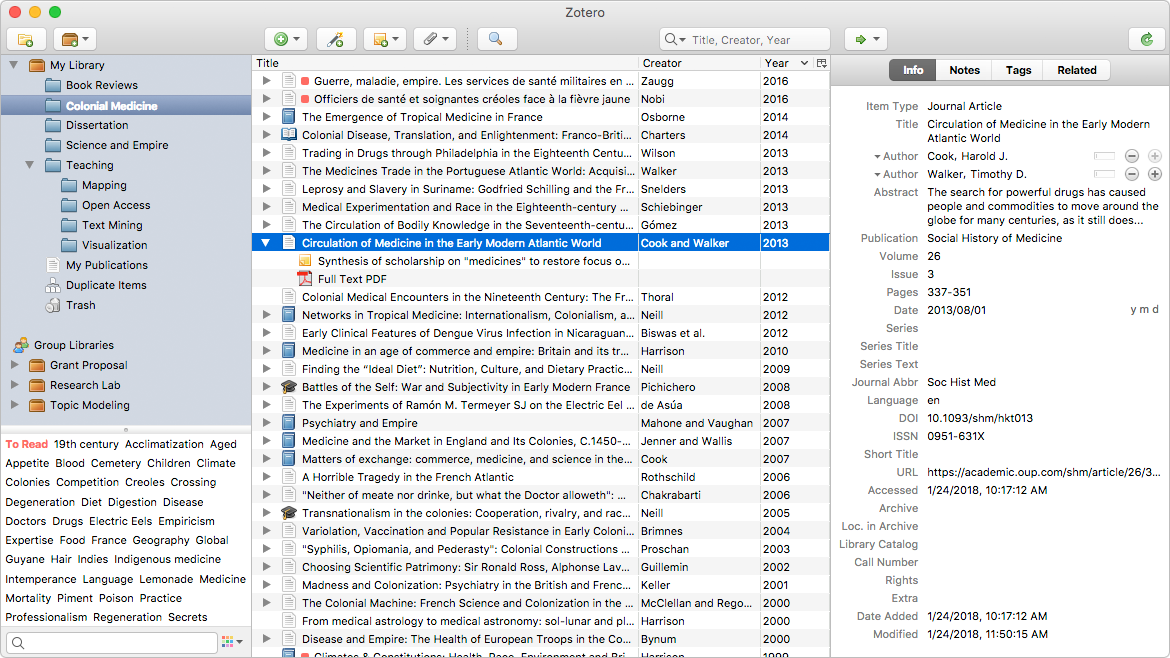
\includegraphics[width=0.8\textwidth]{pictures/zotero.png}
\caption{Zotero基本界面}
\label{fig566}
\end{figure}




\paragraph{(1)常用的功能}
如图(\ref{fig566})所示,Zotero基本分成三栏,左边是分类区,中间是文献区,右边是文献详细信息区。
分类区又分为上下两区,上面称为 Collection,下面则是每篇文献的标签汇总称为Tag。
\begin{itemize}
\item 前往官网下载安装相应版本和插件,并注册帐号。
\item 在 Library 创建 Collection。
\item 选中 Collection 就可以在程序中间文献区导入文献,这样 Zotero 就自动获取文献名、作者、年份等信息。导入文献有两种方式:
\begin{itemize}
\item Link to File: 这种是建立与本地文献链接,不上传到云盘模式。
\item Store Copy of File: 这种是复制到Zotero存贮区上传到云盘模式。请参考多平台、多设备同步。
\end{itemize}
\item 选择一篇文献,在右侧Tags处写上标签,一般多个,如:特别关注的作者、文献中的方法和研究对象。
\item 所有标签就会出现在 第一栏下面区域。首先在 Collection 区域选择 Library,中栏就能呈现所有文献,再在 Tag 区域选中任意标签,就会在中栏筛选出相应的标签。选中多个标签,则是取文献的交集。
\item 通过标签解决了一篇文献多个分类的问题。
\item Collection 中的文献复制有两种方式:
\begin{itemize}
\item 选中 + 拖放:在多个Colletion中复制并保留文献条目; 
\item 选中 + shift + 拖放:从不同Colletion中移动条目。
\end{itemize}
\end{itemize}



\paragraph{(2)文献快速下载与导入}
通过相关的浏览器插件,可以一步实现文献下载和Zotero的导入。但是前提的有,1)Zotero是打开着的;2)自己有文献下载的权限,能把文献下载下来,如果不能,则只会保存一个文献信息,需要后期关联。



\paragraph{(3)多平台、多设备同步}
这是一个非常实用的功能。

\emph{以我为例,主要工作系统是 Ubuntu 系统。但为了实现无纸化办公,我喜欢用微软的 Surface 来阅读文献。而且用 Surface 的笔可以直接在pdf文献上标注,标注也可以同步到主要工作电脑上,非常方便。}

Zotero 自己是有空间同步本地文献的,但是价格太贵。主要可以采用两种方式:1)Zotero +同步盘(任意云盘,软链接);2)Zotero +坚果云WebDAV。推荐后者,详情请参考青柠学术微信公众号专辑,Zotero|打造最佳文献生态。

\paragraph{(4)文献全文检索并自动更新}
还是参考青柠学术Zotero专辑。在“My library”右键有“New Saved Search”。这个可以对文献库中文献进行特定检索,并随着加入的文献自动更新。



\subsection{文献下载}
\begin{itemize}
\item \url{https://bookos-z1.org/}:英文专业书籍下载网站
\item \url{sci-hub.tw}:文献下载网站
\item Zotero + Zotero Connector + Zotero-shortdoi + SCi-Hub: 文献下载标签一条龙,几乎能完成99\%文献下载,参考青柠学术的Zotero专题。
\end{itemize}


\subsection{文献检索与推送——Google学术}
参考:\url{https://scholar.google.com/intl/en/scholar/help.html#overview}



\subsection{Pdf批量全文搜索工具——Recoll}
\begin{itemize}
\item Recoll 网址:\url{https://www.lesbonscomptes.com/recoll/}

\item 参考网址:\url{http://www.linuxdown.net/install/faq/20160318_how_linux_5065.html}
\end{itemize}





\section{自然科学论文写作}
\subsection{摘要(Abstract)}
摘要一般5到6句话。
\begin{itemize}
\item 第一句:大背景;
\item 第二句:领域中有什么问题、我想做什么、有什么是未知的、有什么需要做的;
\item 有些文章不写第一句、第二句
\item 第三句:我用什么方法研究了什么东西;
\item 第四、五句:有什么结果。或加一句分析一下;
\item 最后一句:意义(重要性)。
\end{itemize}


\subsection{引言(Introduction)}
引言的写作直接影响到读者对文章进一步了解的兴趣, 建议包括以下内容\footnote{参考自物理学报的投稿模板}:
\begin{enumerate}
\item 本研究领域背景的综述;
\item 其他学者已有研究成果的详细描述;
\item 陈述为什么需要进行更多的或进一步的研究;
\item 阐述作者本项研究的目的和创新性;
\item 简述本文开展的研究工作;
\item 本项研究结果的意义(可选项)。
\item 特别指出的是, 希望在引言部分介绍和引用国内外期刊中本研究领域的最新研究成果, 以帮助读者清楚了解该领域的最新进展及本文的创新点。
\end{enumerate}



\section{演示文稿(PPT)制作}
图和列表(关键词)



\section{墙报制作}




\section{科研资源}
\subsection{光学相关}
 \begin{itemize}
\item \url{http://toolbox.lightcon.com/}
\end{itemize}







